%
% fourier.tex
%
% (c) 2025 Prof Dr Andreas Müller
%
\documentclass[tikz]{standalone}
\usepackage{amsmath}
\usepackage{times}
\usepackage{txfonts}
\usepackage{pgfplots}
\usepackage{csvsimple}
\usetikzlibrary{arrows,intersections,math}
\begin{document}
	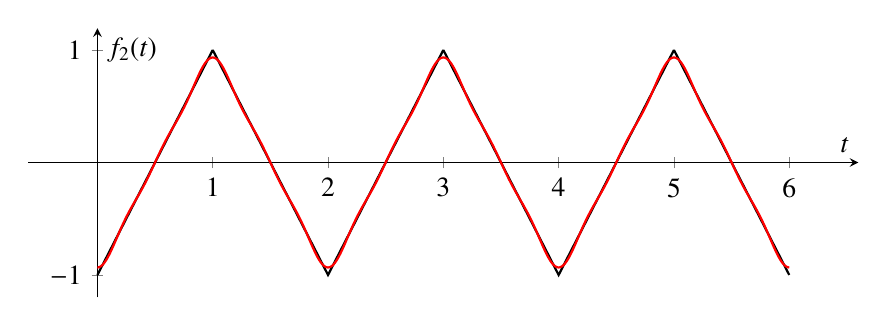
\begin{tikzpicture}
		\begin{axis}[
			axis lines = middle,
			xlabel = {$t$},
			ylabel = {$f_2(t)$},		
			domain=0:6,
			samples=1000,
			xtick={0,1,2,3,4,5,6},
			ytick={-1,0,1},
			enlargelimits,
			width=\textwidth,
			height=5cm
			]
			\addplot[black, thick] {
				abs(mod(x,2) - 1) * (-2) + 1
			};
			
			%\addplot[red, thick, domain=0:6] {
			%	(8/pi^2) * (
			%	sin(deg(pi*x))/1^2
			%	- sin(deg(3*pi*x))/3^2
			%	+ sin(deg(5*pi*x))/5^2
			%	)
			
			\addplot[red, thick, domain=0:6] {
				(-8/pi^2) * (
				  cos(deg(pi*x))/1^2
				+ cos(deg(3*pi*x))/3^2
				+ cos(deg(5*pi*x))/5^2
				)
			};
		\end{axis}
	\end{tikzpicture}
\end{document}
